\chapter{Spazio di memoria}

Non è immediato definire cosa sia la memoria, perché è necessario scegliere un
\textbf{livello di astrazione} a cui fare riferimento: per un programmatore, la memoria potrebbe essere un insieme di variabili tipate;
invece, per un ingegnere elettronico potrebbe essere un insieme di celle elettroniche.

A seconda del livello di astrazione la memoria può essere definita in modi diversi.

\section{Astrazioni di memoria}

Per quanto riguarda le astrazioni a livello software, ci sono pricipalmente tre livelli.

\begin{figure}[ht]
    \centering
    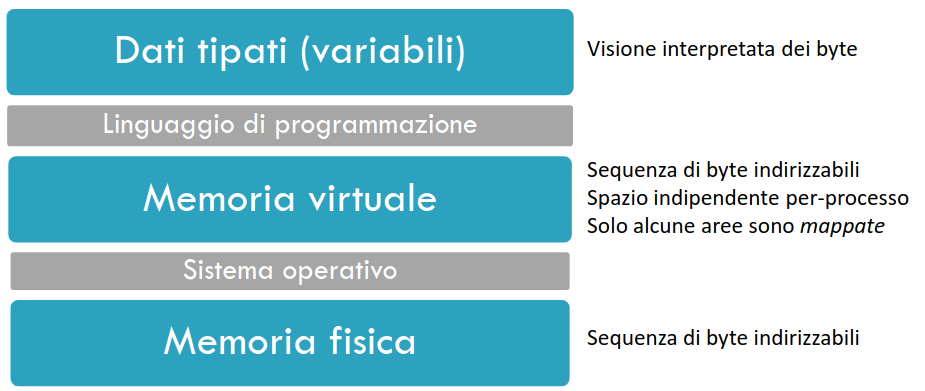
\includegraphics[width=0.75\linewidth]{images/astrazioni.png}
\end{figure}

\subsection{Memoria fisica}

È il livello più basso di astrazione. Ha una struttura semplice: è una \textbf{lunga
sequenza di byte} dove ogni byte ha un \textbf{indirizzo};
il primo byte ha indirizzo 0, il secondo 1, e così via.

È possibile leggere o scrivere dei byte in questa memoria usando delle istruzioni del processore (che parlerà effitivamente con
i banchi di RAM).

\subsubsection{Problematiche dell'utilizzo della memoria fisica}

Questo strato di memoria non è adatto alle esigenze dei sistemi moderni, come
ad esempio la programmazione, perché?

Immaginiamo di avere due programmi in esecuzione nello stesso momento sulla stessa macchina;
entrambi questi programmi devono fare delle operazioni sulla memoria, operando quindi su certi indirizzi di memoria.

Se questi programmi fossero scritti scegliendo gli stessi indirizzi, finirebbero per \textit{"pestarsi i piedi"}.
Da una parte è problematico far convivere applicazioni diverse, assicurandosi che utilizzino indirizzi di memoria diversi;
dall'altra ci sono problemi di sicurezza nell'usare direttamente la memoria fisica: un'applicazione
malevola potrebbe andare a toccare la memoria di un'altra applicazione
influenzandone il comportamento.

Per queste ragioni nessuna applicazione moderna utilizza direttamente la memoria fisica, ma una 
sua astrazione chiamata \textit{memoria virtuale}.

\subsection{Memoria virtuale}

È una astrazione della memoria fisica realizzata dal sistema operativo, che è l'unico componente
che lavora effitivamente sulla memoria fisica.

A livello di \textit{contenuto}, segue la stessa struttura della memoria fisica: è una sequenza di byte indirizzabili.

Però, a differenza della memoria fisica, \textbf{ogni processo di sistema ha uno spazio di memoria indipendente}: ogni programma ha la sua memoria
\textbf{indipendente} ed \textbf{isolata} dalla memoria virtuale degli altri processi.

In questo modo, si evita che i processi \textit{"si pestino i piedi"} o che uno vada a toccare la 
memoria dell'altro.

\subsubsection{Mapping}

Per realizzare questa astrazione si utilizzano dei mapping: ogni area della memoria virtuale è 
mappata a un'area della memoria fisica. Questo processo è realizzato dal sistema operativo.

Ne consegue che è possibile avere lo stesso indirizzo virtuale in due processi diversi, mappati a due indirizzi fisici diversi.

La memoria virtuale non è completamente accessibile, ma solo alcune aree che
effitivamente servono sono mappate.

\subsubsection{Flag di protezione}

La memoria virtuale fornisce delle \textbf{funzionalità di protezione degli accessi}:
si può marcare ciascuna area della memoria virtuale come solo lettura, leggibile/scrivibile, controllare se può contenere codice che può essere eseguito, e così via.

Si può dunque controllare il tipo di accesso che è consentito fare a determinate aree di memoria virtuale.

\subsection{Dati tipati (variabili)}

L'astrazione dei tapi tipati viene realizzata dai linguaggi di programmazione
sopra la memoria virtuale.
Quando dichiaro una variabile, il linguaggio di programmazione si tiene un pezzettino di memoria virtuale per contenere quella variabile.

Quando scrivo (ad esempio) un intero in quella variabile, il linguaggio di programmazione converte quell'intero
in una sequenza di byte per poi metterlo in memoria.

Quando va a leggere quell'intero, viene letta la sequenza di byte dalla memoria per poi riconvertirlo in un intero.

\section{Spazio virtuale Linux userspace}

Andiamo a vedere com'è fatto la memoria virtuale di un processo 
utente su Linux; il kernel avrà uno spazio virtuale diverso.

Quando viene \textbf{lanciato un eseguibile} (binario), viene creato un processo e quell'eseguibile viene
\textbf{caricato in memoria virtuale}.

Il binario contiene varie parti, come quella in cui è contenuta il codice o quella in cui sono contenuti i dati;
tutte queste informazioni vengono caricate in memoria.

Altre aree interessanti in memoria virtuali sono:
\begin{itemize}
    \item \textbf{heap:} contiene tutte le allocazioni dinamiche (\textit{malloc() in C, new() in C++})
    \item \textbf{librerie} esterne importate nel programma
    \item \textbf{stack:} è dove vengono memorizzate le variabili locali e tutta una serie di informazioni
    utilizzate per il flusso di controllo del programma, come gestire le chiamate a funzione
\end{itemize}

\begin{figure}[ht]
    \centering
    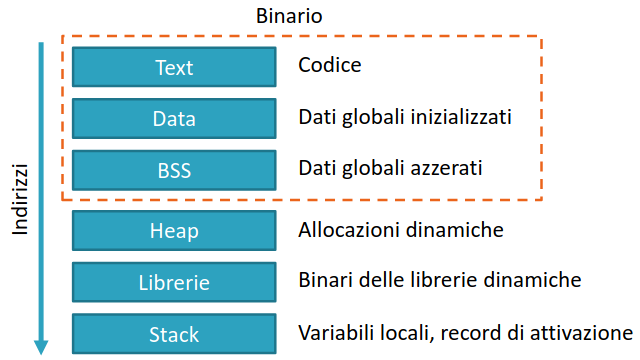
\includegraphics[width=0.75\linewidth]{images/linux-userspace.png}
\end{figure}

Il \textbf{binario} è posizionato ad indirizzi relativamente \textbf{bassi}, mentre lo
\textbf{stack} è l'area che sta ad indirizzi più \textbf{alti}.

\subsection{Un esempio}

In Figura \ref{fig:ex-c} viene mostrato un programma che stampa quattro indirizzi:
\begin{itemize}
    \item indirizzo della funzione main, quindi del codice macchina del programma
    \item indirizzo di una variabile locale
    \item indirizzo di una locazione sull'heap
    \item indirizzo di stack
\end{itemize}
 
\begin{figure}[ht]
    \centering
    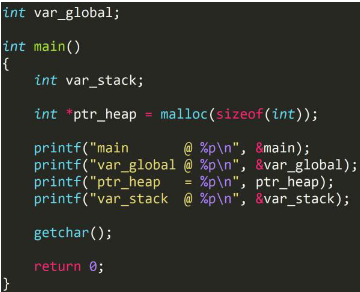
\includegraphics[width=0.65\linewidth]{images/example-1.png}
    \caption{Programma C}
    \label{fig:ex-c}
\end{figure}

In Figura \ref{fig:ex-c2} viene mostrato il risultato dell'esecuzione del programma.s

\begin{figure}[ht]
    \centering
    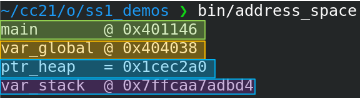
\includegraphics[width=0.75\linewidth]{images/example-2.png}
    \caption{Esecuzione del programma C}
    \label{fig:ex-c2}
\end{figure}

In Linux è possibile vedere il layout della memoria virtuale di un processo usando
il \textit{file system} \texttt{'proc'}: \texttt{/proc} ha una \textit{sub-directory} per
ogni processo del sistema (nominata con l'id del processo nel sistema).

Ciò che viene fatto in Figura \ref{fig:ex-c3} è stato usare \texttt{pgrep} per trovare l'id associato al processo \textit{address\_space} (il
programma C).

In ogni linea:
\begin{itemize}
    \item il primo numero è l'indirizzo di partenza in esadecimale, e dopo '-' c'è l'indirizzo di fine
    \item dopo ci sono i flag di protezione (\texttt{r, rw, x})
\end{itemize}

\begin{figure}[ht]
    \centering
    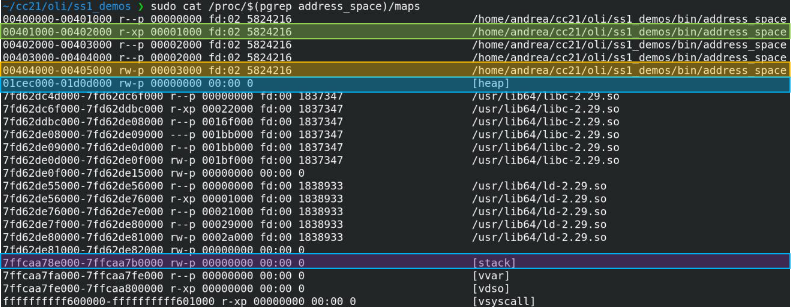
\includegraphics[width=1\linewidth]{images/example-3.png}
    \caption{Layout della memoria virtuale del processo}
    \label{fig:ex-c3}
\end{figure}

L'indirizzo del  \textcolor{green}{\textbf{\textit{main}}} è leggibile ed eseguibile.

La \textcolor{orange}{\textbf{\textit{variabile globale}}} è leggibile e scrivibile; 
lo stesso vale per l'\textcolor{blue}{\textbf{\textit{heap}}}.

Dopo ci sono una serie di mapping di \textit{libc} e \textit{ld}, una serie di librerie standard
caricate in tutti i processi. Se il processo utilizza delle liberie aggiuntive saranno caricate in questa zona.

Infine, negli indirizzi più alti, si trova lo \textcolor{purple}{\textbf{\textit{stack}}}.


